\documentclass{beamer}
\usepackage[spanish ]{babel}
\usepackage{multicol} % indice en 2 columnas
\usepackage[latin1]{inputenc}
\usepackage{graphicx}
\usepackage{media9}
\usepackage{cite}
\usepackage{array}
\usepackage{booktabs}
\usepackage{subfigure}
\usepackage{amsmath,amssymb,latexsym}
\usetheme{Warsaw}
\usepackage{hyperref}
%\usecolortheme{crane} 
%\usecolortheme{crane}
\definecolor{colorEND}{RGB}{40,0,130} % define color
\setbeamercolor*{palette primary}{use=structure,fg=white,bg= colorEND!50}
\setbeamercolor*{palette quaternary}{use=structure,fg=white,bg=colorEND}
\beamertemplatenavigationsymbolsempty % remove navigation bar 
\logo{
\includegraphics[width=1cm]{endlabiconcopia}\vspace{-0.3cm} \hspace{0.1cm}} % logo end

\useoutertheme{shadow}
\useinnertheme{rectangles}
\setbeamertemplate{navigation symbols}{} % quitar simbolitos

\title[CINEND]{Ciclo de Cine}
\author[G. A. Moreu Vijande]
{G. A. Moreu Vijande}
\institute[Universidad \& de Granada]
{
\small \url{https://github.com/gmoreuv/primer}
 \begin{center}
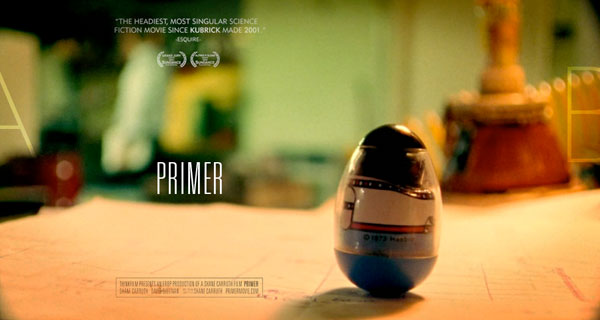
\includegraphics[width=62mm]{primertop}
\end{center}
}
\date{}

\begin{document}

\frame{\titlepage}
\begin{frame}
\begin{columns}[t]
    \column{0.5\textwidth}
\begin{figure}[h]
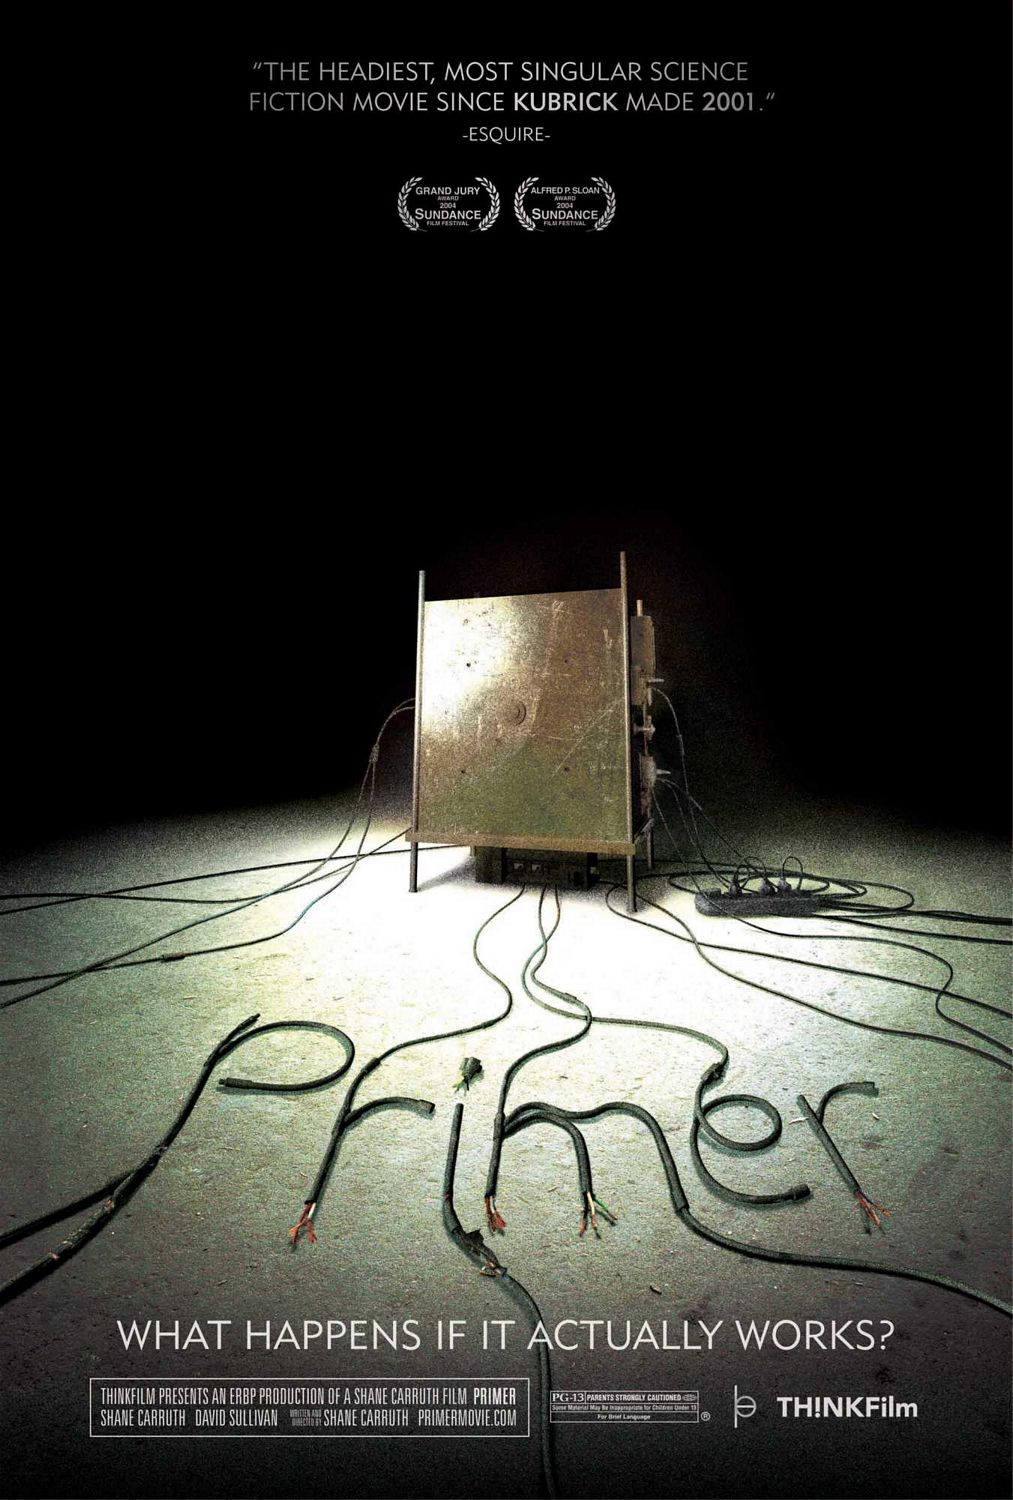
\includegraphics[width=0.8\textwidth]{primer_poster}
\end{figure}
 \column{0.5\textwidth}
\begin{figure}
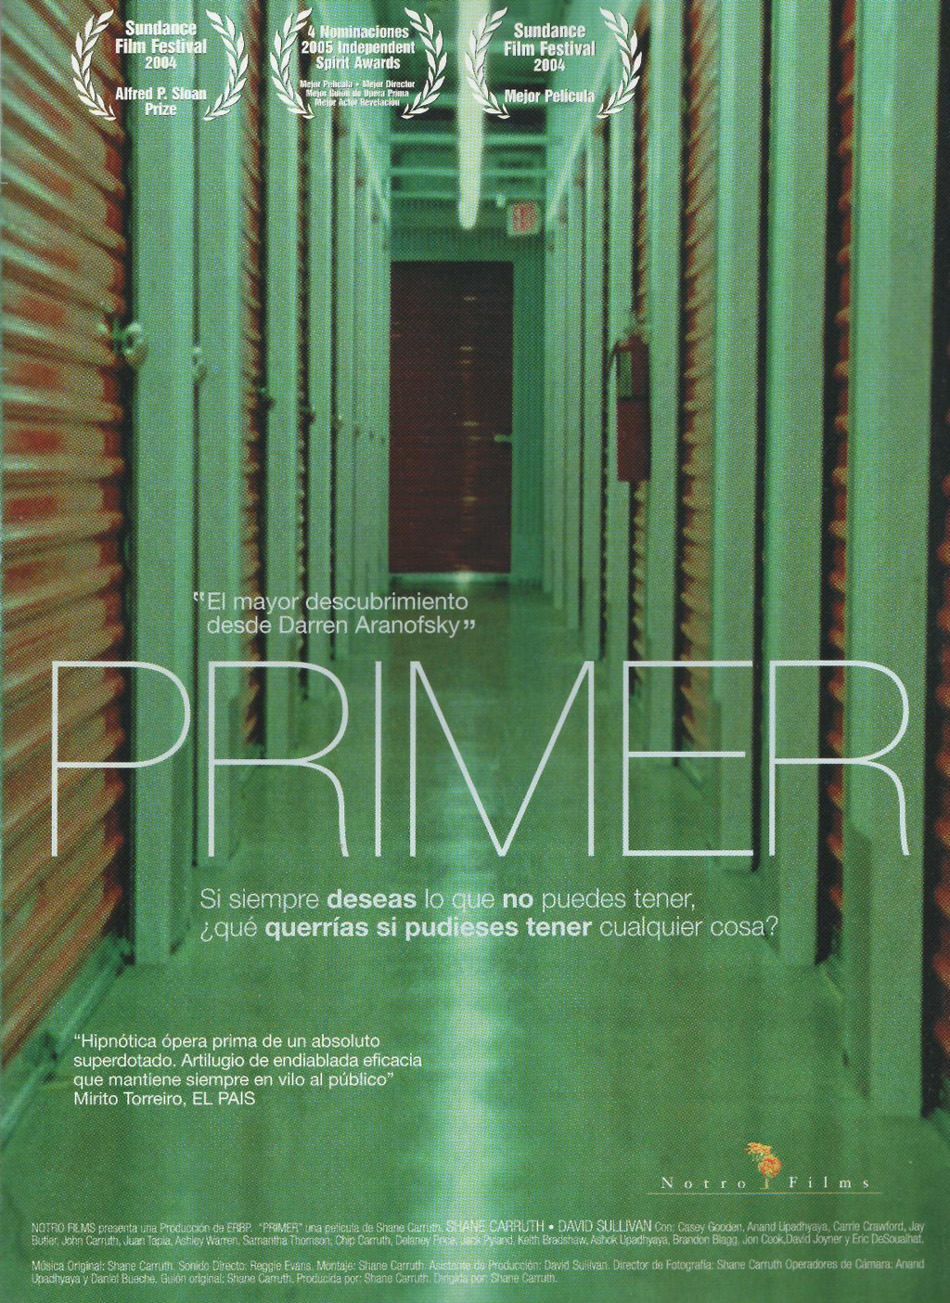
\includegraphics[width=0.86\textwidth]{primer_poster2}
\end{figure}
\end{columns}
\end{frame}

%\begin{frame}
%\frametitle{Indice}
%\tableofcontents
%\end{frame}

\section{PRIMER}
\subsection{Sinopsis}

\begin{frame}[allowframebreaks]
  \frametitle{Sinopsis}
  \begin{block}{Filmaffinity}
  \begin{itemize}
  	\item Cuatro hombres trabajan en un garaje construyendo aparatos altamente complejos. En parte por accidente y en parte por su pericia, descubren un mecanismo dotado de poderes que les permite conseguir casi todo lo que quieran. Se trata de un hallazgo que podr�a cambiar el mundo, pero que pondr� a prueba las relaciones entre sus inventores.
	\item \textbf{Nota media de los usuarios}: 6.2/10  (24.092).
\end{itemize}
\end{block}

\begin{block}{IMDB}
\begin{itemize}
\item  At night and on weekends, four men in a suburban garage have built a cottage industry of error-checking devices. But, they know that there is something more. There is some idea, some mechanism, some accidental side effect that is standing between them and a pure leap of innovation. And so, through trial and error they are building the device that is missing most. However, two of these men find the device and immediately realize that it is too valuable to market. The limit of their trust in each other is strained when they are faced with the question, If you always want what you can't have, what do you want when you can have anything?
\item \textbf{Nota media de los usuarios}: 7.0/10  (68.421 votos).
\end{itemize}
\end{block}
\end{frame}

\subsection{Ficha T�cnica}
\begin{frame}
\frametitle{Ficha T�cnica}
	\begin{itemize}
		\begin{columns}[t]
   			\column{0.65\textwidth}
				\item []
				\item \textbf{Aaron} $\rightarrow$ \small{Interpretado por \textit{Shane Carruth}} $\rightarrow$ \small{EL MORENO}
				\item[]
				\item[]
				\item[]
				\item \textbf{Abe} $\rightarrow$ Interpretado por \textit{David Sullivan} $\rightarrow$  \ \ \ \ EL RUBIO
			 \column{0.3\textwidth}
				\begin{figure}
					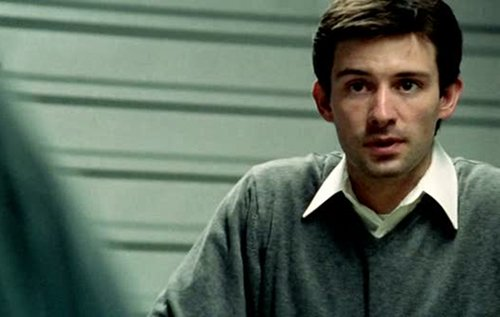
\includegraphics[width=0.76\textwidth]{aaron}
				\end{figure}
				\begin{figure}[h]
					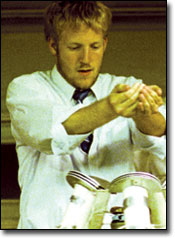
\includegraphics[width=0.6\textwidth]{abe}
				\end{figure}
		\end{columns}
	\end{itemize}
\end{frame}

\subsection{Consejos para una correcta visualizaci�n}
\begin{frame}[allowframebreaks]
\frametitle{Consejos para una correcta visualizaci�n}
	\begin{itemize}
		\item Ponte c�modo.
		\item Vas a ver una pel�cula densa en cuanto a argumento e informaci�n.
		\item Pon el m�vil en avi�n.
		\item Presta atenci�n.
		\item Sigue prestando atenci�n.
		\item Muchas cosas no se cuentan, se intuyen o se explican al final.
		\item Si te pierdes, no te preocupes, la persona de tu lado es probable que tambi�n se haya perdido.
		\item Atenci�n a la \textit{No Linealidad-Lineal}
		\newpage
		\item Al final, pondr� este gr�fico \textbf{levemente} explicativo.
		\begin{figure}[h]
			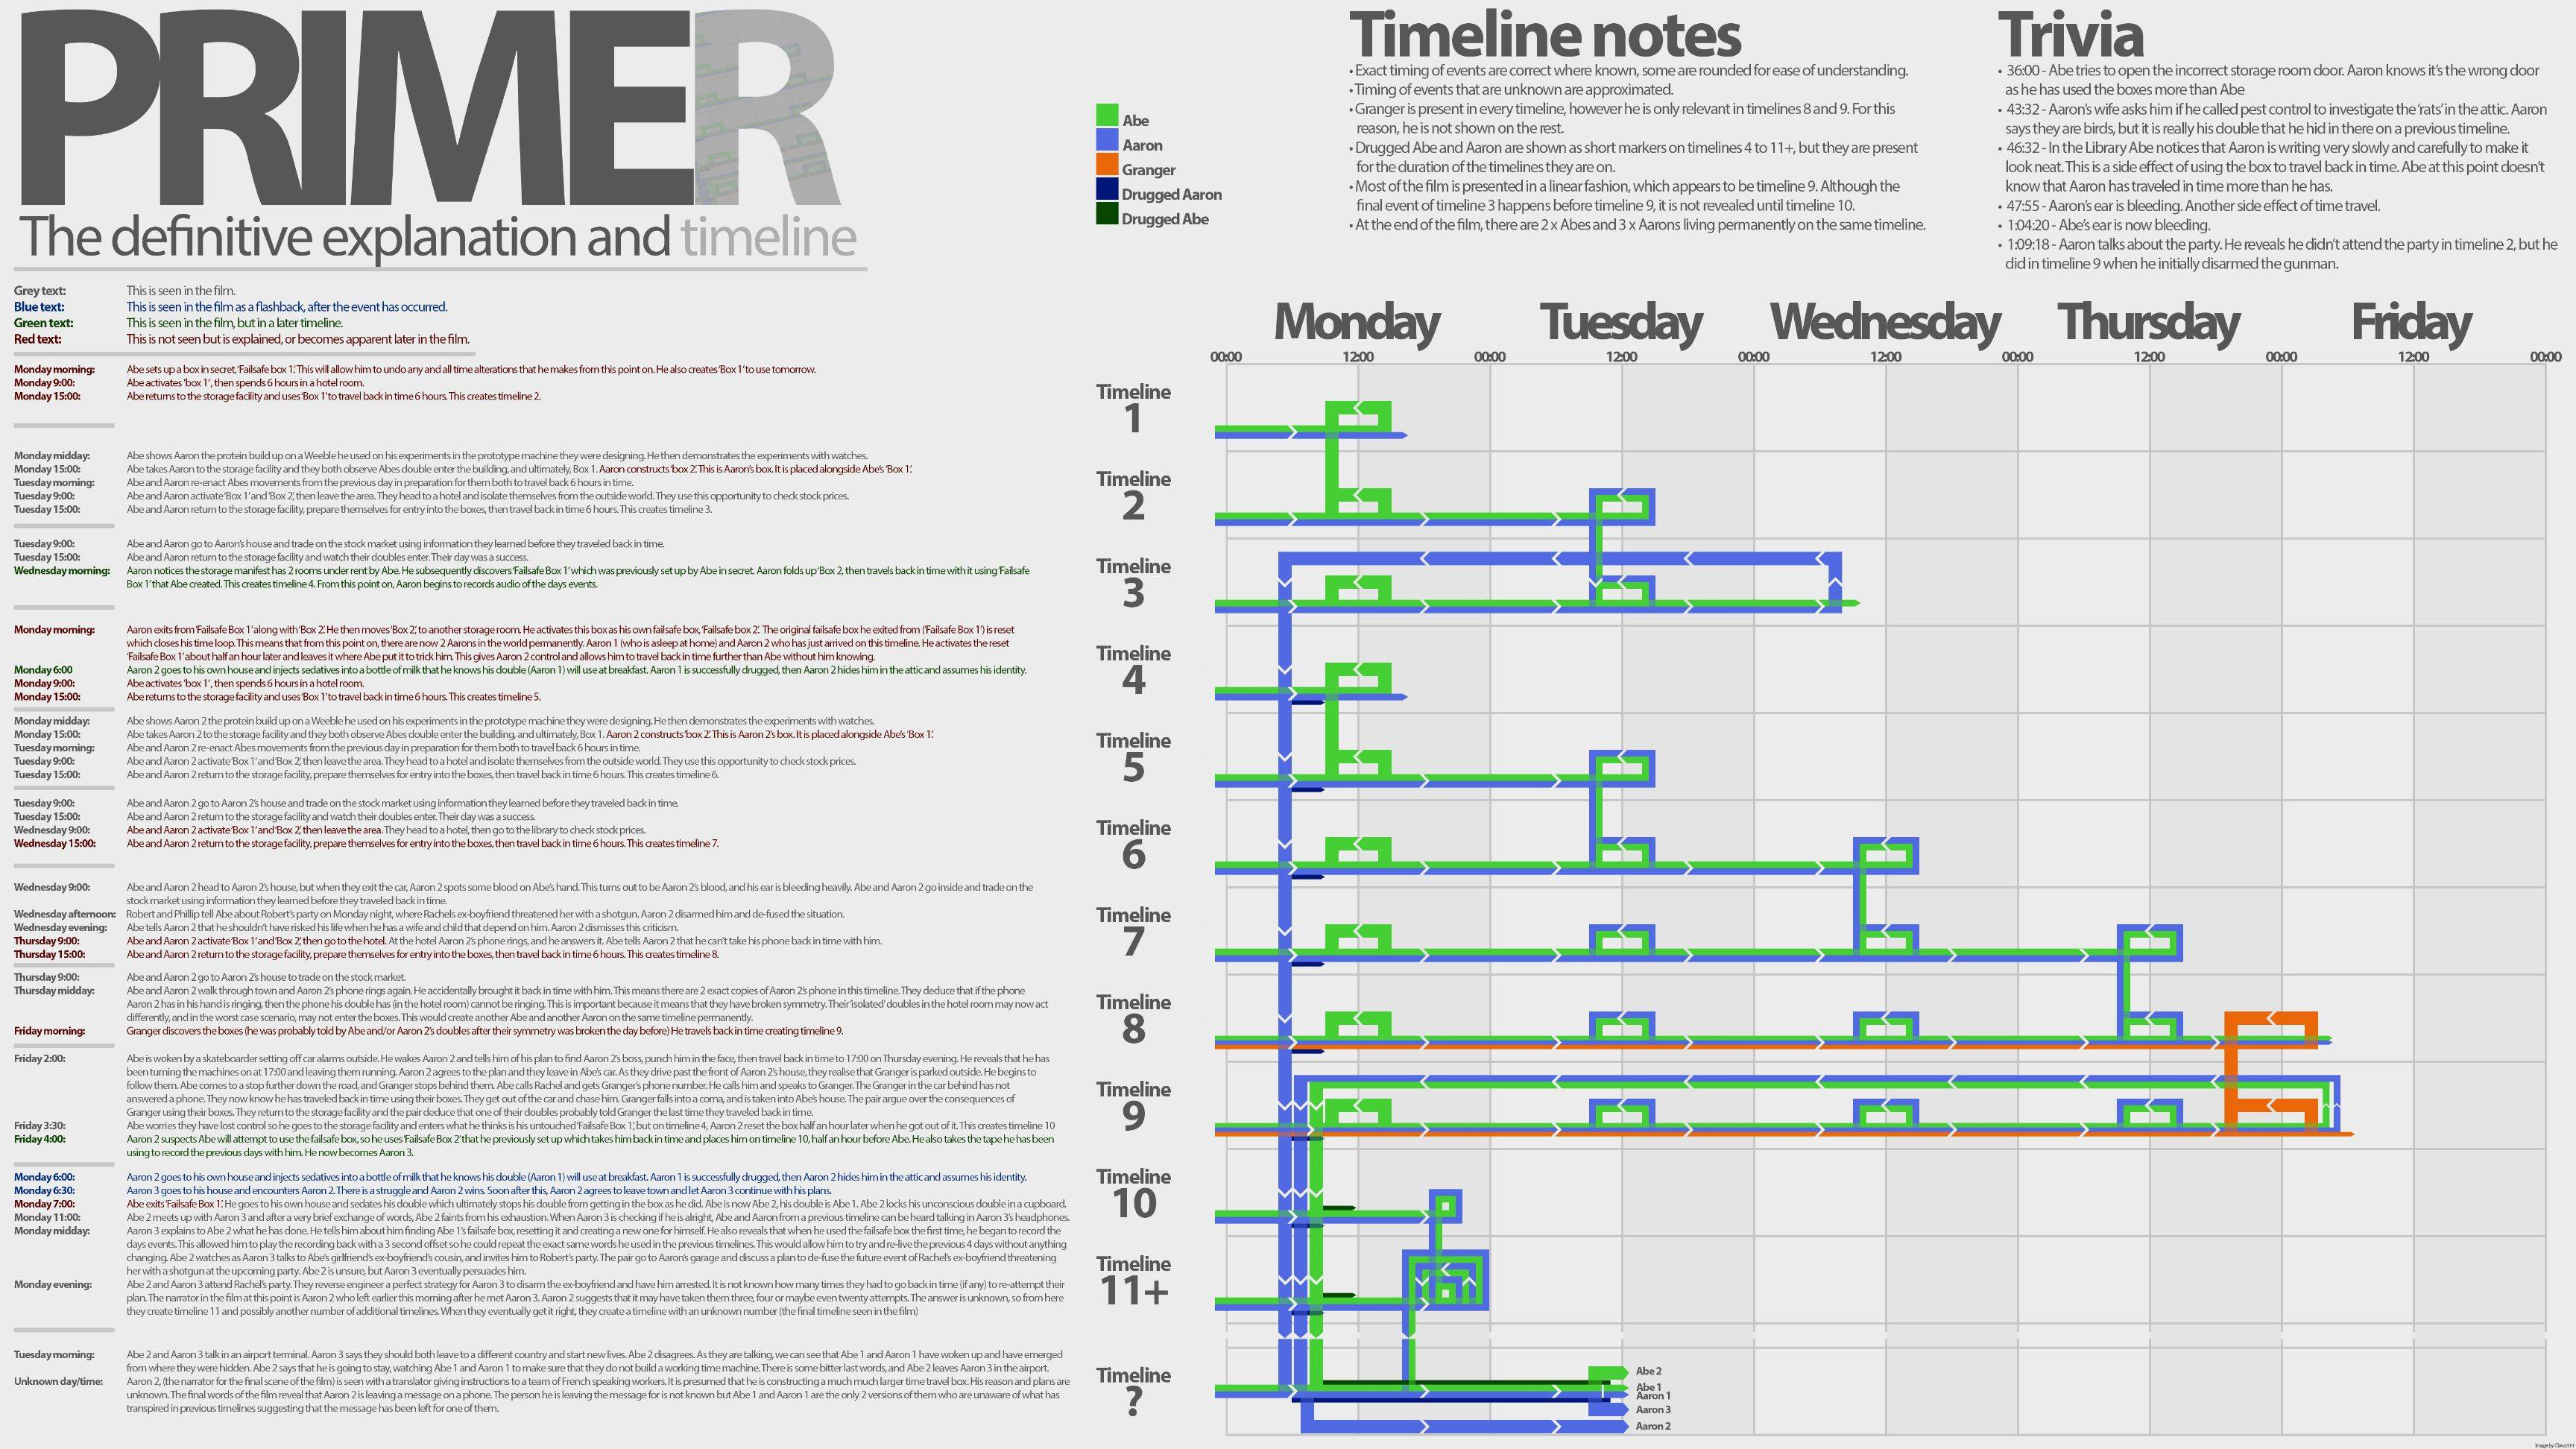
\includegraphics[width=0.85\textwidth]{timeline01}
		\end{figure}
		\newpage
		\item Pero no os preocup�is si os sent�s as�:
		\begin{figure}[h]
			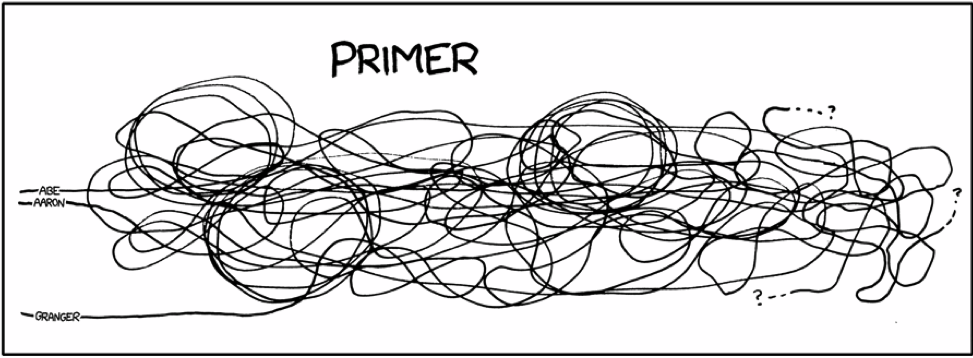
\includegraphics[width=0.85\textwidth]{timeline02}
		\end{figure}
	\end{itemize}
\end{frame}


\subsection{Opciones de visualizaci�n}
\begin{frame}[allowframebreaks]
\frametitle{Opciones de visualizaci�n}
	\begin{block}{\huge{Idioma: Ingl�s $\rightarrow$ Subt�tulos: Espa�ol}}
		\begin{itemize}
			\item \textbf{PROS}
				\begin{itemize}
					\item Mayor calidad de audio
					\item Idioma original
					\item Siempre se aprende/mejora el ingl�s
				\end{itemize}
			\item \textbf{CONTRAS}
				\begin{itemize}
					\item Leer, escuchar y retener mucha informaci�n no es f�cil
					\item Alto desv�o de atenci�n al tener que leer
					\item Es posible no apreciar todos los detalles del argumento
					\item Es bastante probable que te enteres de poco
				\end{itemize}
		\end{itemize}
	\end{block}
	
	\begin{block}{\huge{Idioma: Espa�ol}}
		\begin{itemize}
			\item \textbf{PROS}
				\begin{itemize}
					\item Al no tener que leer, prestas m�s atenci�n a la composici�n de la escena, a los peque�os detalles, a lo que te cuentan en la pel�cula y a lo que no te cuentan en ella
				\end{itemize}
			\item \textbf{CONTRAS}
				\begin{itemize}
					\item Peor calidad de audio
					\item Siempre existen problemas de traducci�n al doblar
					\item No se aprende ingl�s
				\end{itemize}
		\end{itemize}
	\end{block}
\end{frame}

\subsection{Premios y Galardones}
\begin{frame}
\frametitle{Premios y Galardones}
	\begin{itemize}
		\item Gran Premio del Jurado de \textbf{Sundance} en 2004.
		\item Premio \textit{Alfred P. Sloan} para pel�culas de tem�tica cient�fica y tecnol�gico en 2004.
		\item Mejor director y gui�n en el festival de \textbf{Nantucket} en 2004
		\item Mejor pel�cula en el Festival Internacional de Londres de Ciencia Ficci�n en 2005.
	\end{itemize}
\end{frame}


\end{document}